\begin{figure*}
  %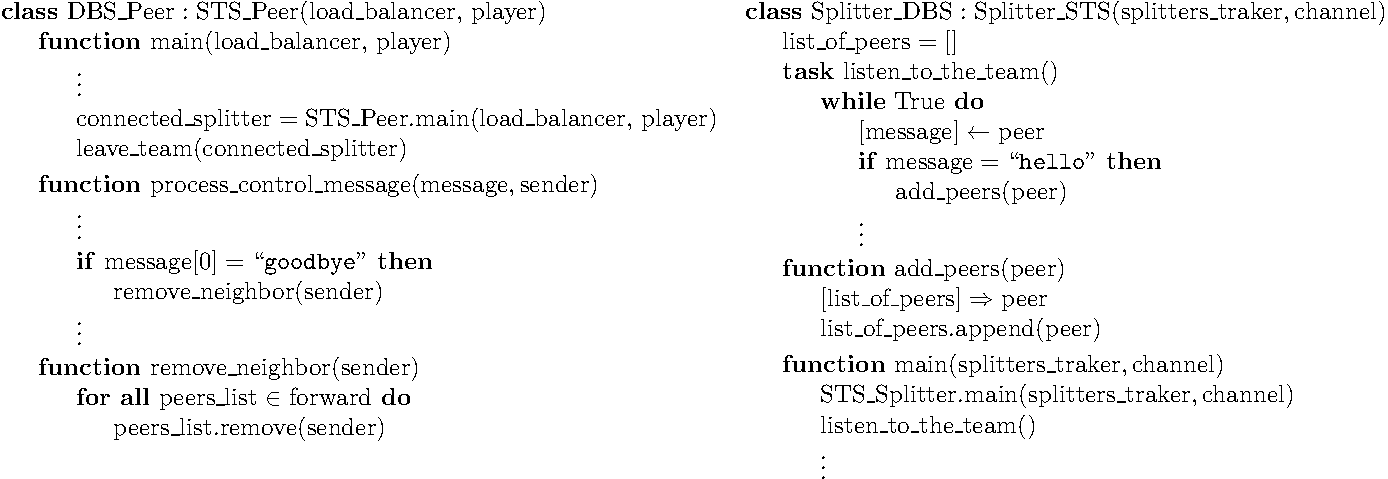
\includegraphics[width=0.55\textwidth]{leaving}
  \fig{300}{4cm}{leaving}
  \caption{Tasks run when an peer $P_o$ wants to leave its
    team. $P_k$ is a neighbor of $P_o$.\label{fig:leaving}}
\end{figure*}
An outgoing peer $P_o$ (see Fig.~\ref{fig:leaving}) must to: (1) say
$[\mathtt{goodbye}]$ to $S$ and to $T^o$ (in this order), (2)
relay any pending (received but yet not sent) chunks, and (3) wait for
a $[\mathtt{goodbye}]$ from $S$, which performs $T = T \setminus
P_o$. In case of a timeout, $P_o$ resets the leaving procedure,
for a maximum number of times.

When a $P_k$ receives a $[\mathtt{goodbye}]$ from $P_o$, $P_k$
removes $P_o$ from its neighbors set, by running $T^k = T^k
\setminus P_o$.
